 \paragraph*{Пример\\}
 
\hspace*{\parindent}Рассмотрим нахождение DH параметров на конкретной задаче:\\

Пусть имеется такая система:\\
\begin{center}
    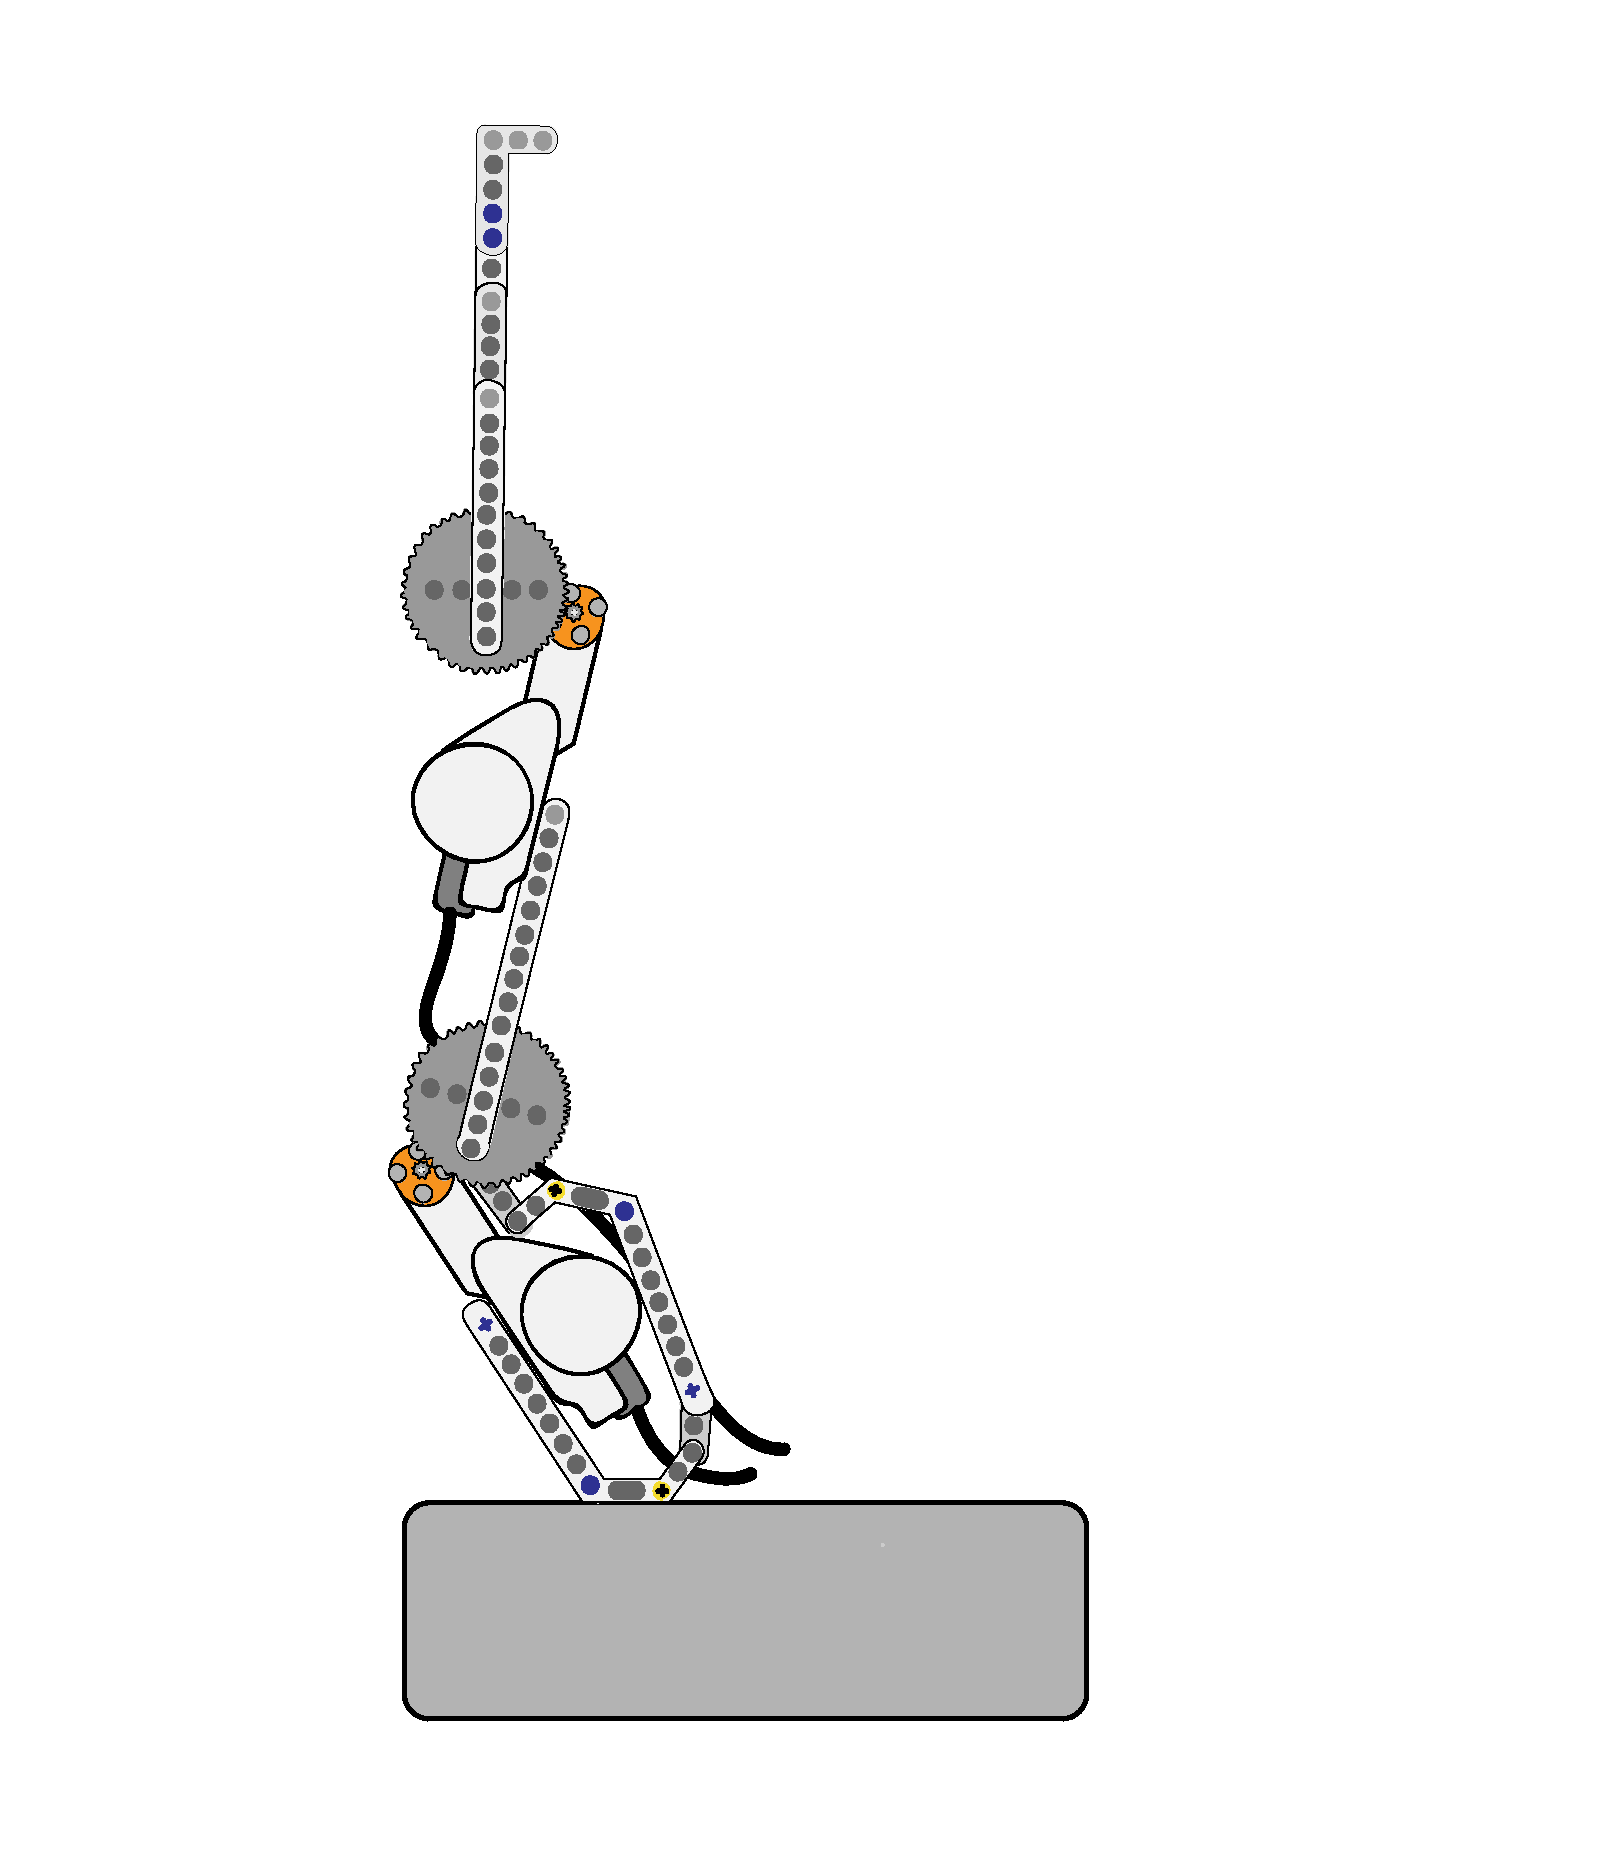
\includegraphics[width=0.6\textwidth]{DH1.pdf}\\
    Рисунок 2.1.2 Система для определения DH параметров.\\
\end{center}


\hspace*{\parindent}Расставляются положения DH-параметров по правилам, описанным выше:\\ 
\hspace*{\parindent}В начале определяются параметры $a_i$: системы $x_0y_0z_0$ и $x_1y_1z_1$ совпадают, следовательно сдвигов нет, далее рассматривается пара систем $x_1y_1z_1$ и $x_2y_2z_2$ здесь ость $z_2$ лежит в плоскости перпендикулярной рассматриваемому виду и располагается в направлении "от нас", её нулевая координата соответственно совпадает с нулевыми координатами $x_2$ и $y_2$, а значит $a_1$ определяется как расстояние от пересечения $x_1z_1$ до  $x_2y_2$ по оси $x_2$, следующее смещение между осями $z_2$ $z_3$ и $z_3$ $z_4$ выполняется аналогично, они направлены "от нас" и лежат в перпендикулярной плоскости, их начала лежат на пересечении двух других осей, соответственно получаются значения $a_2$ и $a_3$.\\
\hspace*{\parindent}Далее коэффициенты смещения $d_i$: имеется только смещение $d_1$ (поскольку остальные системы по осям $z_i$ не имеют сдвигов) от первой системы до второй.\\
Углы $\alpha_i$ определяются как поворот текущей оси $x_i$ от оси $z_{i-1}$ до оси $z_{i}$. Например, для первого звена ось $z_0$ направлена вверх, а $z_1$ от нас. Значит, поворот был на угол $\frac{\pi}{2}$. \\
\hspace*{\parindent}Углы $\theta_i$ определяются как углы вращения на сочленениях: можно заметить, что при переходе от первой системы ко второй производится дополнительный поворот на угол $\frac{\pi}{2}$, что также заносится в параметр, остальные углы подобного дополнительного вращения не имеют.\\
\begin{center}
    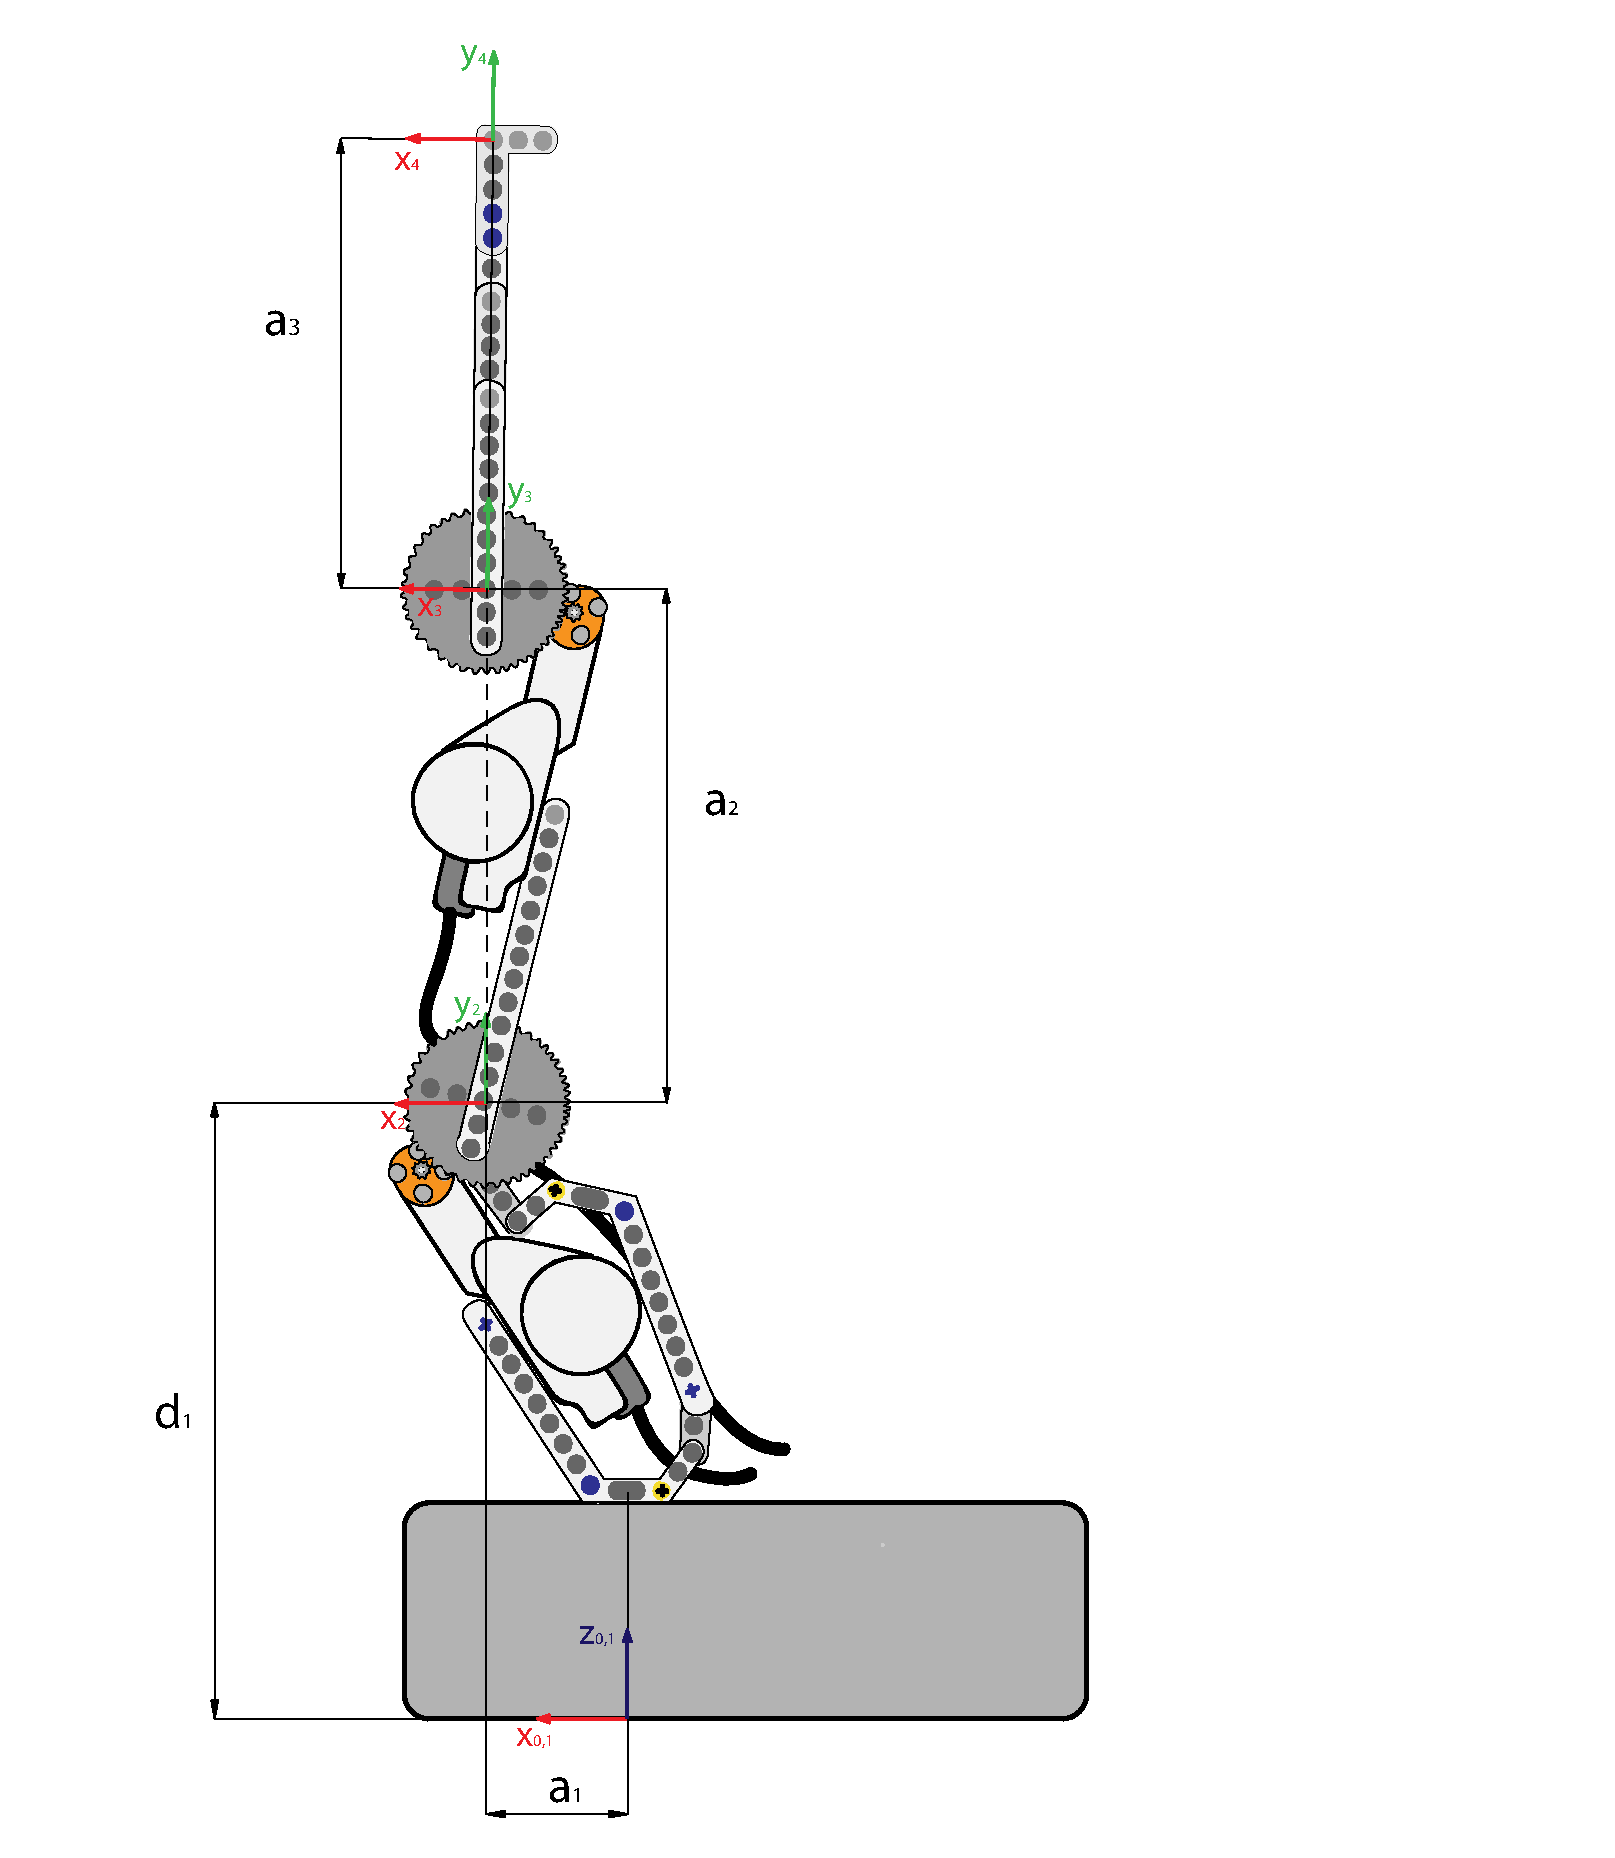
\includegraphics[width=0.575\textwidth]{DH2.pdf}\\
    Рисунок 2.1.3 Система с обозначенными DH параметрами.\\
\end{center}



\begin{table}[h!]
\hspace*{\parindent}Далее измеряются их значения и заносятся в соответствующую таблицу:\\
\begin{center}
\begin{tabular}{|c|c|c|c|c|}
\hline
Звено i & $a_i$ & $\alpha_i$ & $d_i$ & $\theta_i$ \\
\hline
1 & $a_1$ & $\frac{\pi}{2}$ & $d_1$ & $\theta_1$\\
\hline
2 & $a_2$ & 0 & $d_2$ & $\theta_2$ + $\frac{\pi}{2}$\\
\hline
3 & $a_3$ & 0 & $d_3$ & $\theta_3$\\
\hline
\end{tabular}
\end{center}
\end{table} 
\begin{center}
$a_1$ = 0,06 м;  $a_2$ = 0,15 м;  $a_3$ = 0,145 м; \\
$d_1$ = 0,163 м;  $d_2$ = 0 м;  $d_3$ = 0 м \\
\end{center}
\hspace*{\parindent}Подставив все параметры Денавита-Хартенберга для модели, представленной на рис.2.1.1, получим частный случай при n=3 матриц однородного преобразования:\\

\begin{equation*}\label{eq:model}
T_1^0 = 
     \begin{bmatrix}
    cos{\theta_1} & 0 &  -sin{\theta_1} & 0 \\
    sin{\theta_1} & 0 &  cos{\theta_1} & 0 \\
    0 & -1 & 0 & d_1\\
    0 & 0 & 0 & 1\\
    \end{bmatrix}
    ,
\end{equation*} 

\begin{equation*}\label{eq:model}
T_2^1 = 
     \begin{bmatrix}
    cos{(\theta_2 + \frac{\pi}{2})} & -sin{(\theta_2 + \frac{\pi}{2})} & 0 & a_2 cos{(\theta_2 + \frac{\pi}{2})} \\
    sin{(\theta_2 + \frac{\pi}{2})} & cos{(\theta_2 + \frac{\pi}{2})} & 0 & a_2 sin{(\theta_2 + \frac{\pi}{2})}\\
    0 & 0 & 1 & 0\\
    0 & 0 & 0 & 1\\
    \end{bmatrix}
    ,
\end{equation*} 

\begin{equation*}\label{eq:model}
T_3^2 = 
      \begin{bmatrix}
    cos{\theta_3 } & -sin{\theta_3} & 0 & a_3 cos{\theta_3} \\
    sin{\theta_3} & cos{\theta_3} & 0 & a_3 sin{\theta_3}\\
    0 & 0 & 1 & 0\\
    0 & 0 & 0 & 1\\
    \end{bmatrix}
    ,
\end{equation*}  